\section{Auswertung}
	

	\subsection{Magnetfelder}
		
		\noindent
		Die Magnetfeldstärke einer Helmholtzspule berechnet sich nach der Formel:
		\begin{equation}
			B = \mu_0 \frac{8IN}{\sqrt{125}R}.
		\end{equation}		
		Mit den Windungszahlen der Spulen $N$ und dem Radius $R$ der Spulen:
		\begin{align*}
			R_\text{Sweep} = \SI{16.39}{\centi\metre}			\quad   &N_\text{Sweep}    = 11		\\
			R_\text{Horizontal} = \SI{15.79}{\centi\metre}		\quad 	&N_\text{Horizontal} = 154  \\
			R_\text{Vertikal} = \SI{11.735}{\centi\metre}		\quad	&N_\text{Vertikal} = 20
		\end{align*}
		lässt sich aus den Stromstärken aus Tabelle (\ref{tab:Daten1}) und (\ref{tab:Daten2}) die gesamt horizontalkomponente des Magnetfeldes nach
		\begin{equation*}
			B_\text{Gesamt} = B_\text{Sweep} + B_\text{Horizontal}
		\end{equation*} 
		berechnen. Diese Ergebnisse für diese Berechnung sind auch in Tabelle(\ref{tab:Daten2}) eingetragen.
		Die Stromstärke der Vertikal-Spule bei dem der Effekt des Erdmagnetfeldes minimal war, wurde bei \SI{0.23}{\ampere}  gemessen.
		Danach berechnet sich die Erdmagnetfeldstärke zu \SI{35.24}{\micro\tesla}
		
	\subsection{Gyromagnetische Faktoren}
		
		\noindent
		Die Formel(\ref{eqn:zeeman}) lässt sich zu 
		\begin{equation*}
			B = \frac{\hbar}{g_F \, \mu_B} \cdot \omega
			\label{eqn:steig}
		\end{equation*}
		umstellen. In Abbildung(\ref{fig:Daten}) ist die Magnetfeldstärke gegen die RF-Frequenz gezeichnet.
		Hier lässt sich nun die Steigung der beiden Geraden mittels Gleichung(\ref{eqn:steig}) als $ m = \frac{\hbar}{g_F \, \mu_B}$ identifizieren.		
		Diese Steigung lässt sich wiederum zum gyromagnetischen Faktor
		\begin{equation}
		 	g_F = \frac{\hbar}{m \mu_B}
			\label{eqn:gyro}
		\end{equation}
		umstellen.		

		\begin{figure}[H]
			\centering
			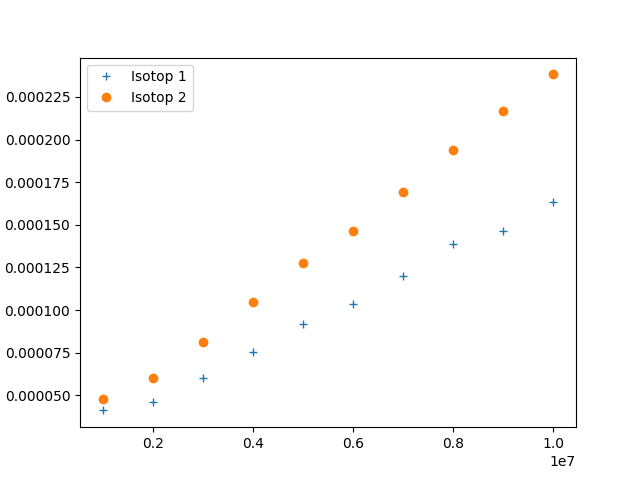
\includegraphics[width=0.7\textwidth]{build/Magnetfeld.png}
			\caption{Die gemessenen Daten aus Tabelle(\ref{tab:Daten}) geplotted mit den berechneten linearen Regressionen.}
			\label{fig:Daten} 
		\end{figure}

		\noindent
		Die Parameter der beiden Regressionen wurden zu:
		\begin{align*}
			m_1 &= \SI{1.42(0.04)e-10}{\tesla\per\hertz}  &b_1= \SI{2.08(0.22)}{\tesla}\\
			m_2 &= \SI{2.17(0.04)e-10}{\tesla\per\hertz}  &b_2= \SI{1.92(0.23)}{\tesla}
		\end{align*}
		bestimmt. Werden diese Steigungen nun in Gleichung(\ref{eqn:gyro}) eingesetzt, ergit sich für die die gyromagnetischen Faktoren:
		\begin{align*}
			&\text{Isotop 1:} \quad g_\text{F} = \num{0.504(0.013)}\\		
			&\text{Isotop 2:} \quad g_\text{F} = \num{0.329(0.006)}			
		\end{align*}

		\begin{table}[h]
			\begin{center}
				\begin{tabular}{c c c  }% c}
					\toprule
						{$\omega_\text{RF} \mathbin{\scalebox{1.5} / } \si{\mega\hertz}$} & {$I_\text{Sweep,1}  \mathbin{\scalebox{1.5} / } \si{\ampere}$} & 
          				{$I_\text{Sweep,2} \mathbin{\scalebox{1.5} / } \si{\ampere}$}\\
					\midrule
 					0.1	& 0.682 & 0.795\\
					0.2 & 0.475 & 0.710\\
					0.3 & 0.710 & 1.060\\
					0.4 & 0.237 & 0.715\\
					0.5 & 0.210 & 0.805\\
					0.6 & 0.265 & 0.970\\
					0.7 & 0.240 & 1.065\\
					0.8 & 0.405 & 0.887\\ 
					0.9 & 0.245 & 0.687\\
					1.0 & 0.385 & 0.750\\
					\bottomrule
				\end{tabular}				
				\caption{Tabelle der RF Frequenzen und den gemessenen Stromstärken der Sweep-Spule.}
			\end{center}
			\label{tab:dat1}
		\end{table}

		\begin{table}[h]
			\begin{center}
				\begin{tabular}{c c c c}
					\toprule
          				 {$I_\text{Hor,1} \mathbin{\scalebox{1.5} / } \si{\ampere}$} &  {$I_\text{Hor,2} \mathbin{\scalebox{1,5} / } \si{\ampere}$} &
						 {$ B_1 \mathbin{\scalebox{1.5} /} \si{\micro\tesla}$} & {$ B_2 \mathbin{\scalebox{1.5} /} \si{\micro\tesla} $}\\
					\midrule
					0.00 & 0.00 &  41.1 &  47.9 \\
					0.02 & 0.02 &  46.6 &  60.3 \\
					0.02 & 0.02 &  60.3 &  81.5 \\
					0.07 & 0.07 &  75.6 & 104.5 \\
					0.09 & 0.09 &  91.6 & 127.5 \\
					0.10 & 0.10 & 103.6 & 146.2 \\
					0.12 & 0.12 & 119.7 & 169.5 \\
					0.13 & 0.16 & 138.4 & 193.8 \\
					0.15 & 0.20 & 146.3 & 216.5 \\
					0.16 & 0.22 & 163.5 & 238.1 \\
					\bottomrule
				\end{tabular}				
				\caption{Tabelle der Stromstärke in der Horizontalspule und der gesamt Magnetfeldstärke in horizontal Richtung.}
			\end{center}
			\label{tab:dat2}
		\end{table}
	\subsection{Kernspin}
		
		\noindent
		Der Kernspin der Isoptope lässt sich mittels 
		\begin{equation}
			I =\frac{1}{2} \left| \frac{g_\text{J}}{g_\text{F}} -1 \right|
		\end{equation}
		berechnen. Hier ist $g_\text{F}$ der Landé-Faktor.
		Werden die berechneten gyromagnetischen Faktoren $g_\text{J}$, in diese Formel eingesetzt, ergibt sich für die Kernspins:
		\begin{align}
			&I_1 = \num{1.48(0.05)}\\
			&I_2 = \num{2.54(0.05)}
		\end{align}

		
	\subsection{Isotopenverhältnis}
		
		\noindent
		Zur Bestimmung des Isotopenverhältnisses wurde bei einer RF Frequenz von \SI{100}{\kilo\hertz} die Peak tiefe der Magnetfeldstärke abgelesen. Da die Peaktiefe auch proportional zum Isotopenverhältnis der beiden RB Isotope.
		
		\begin{figure}[H]
			\centering
			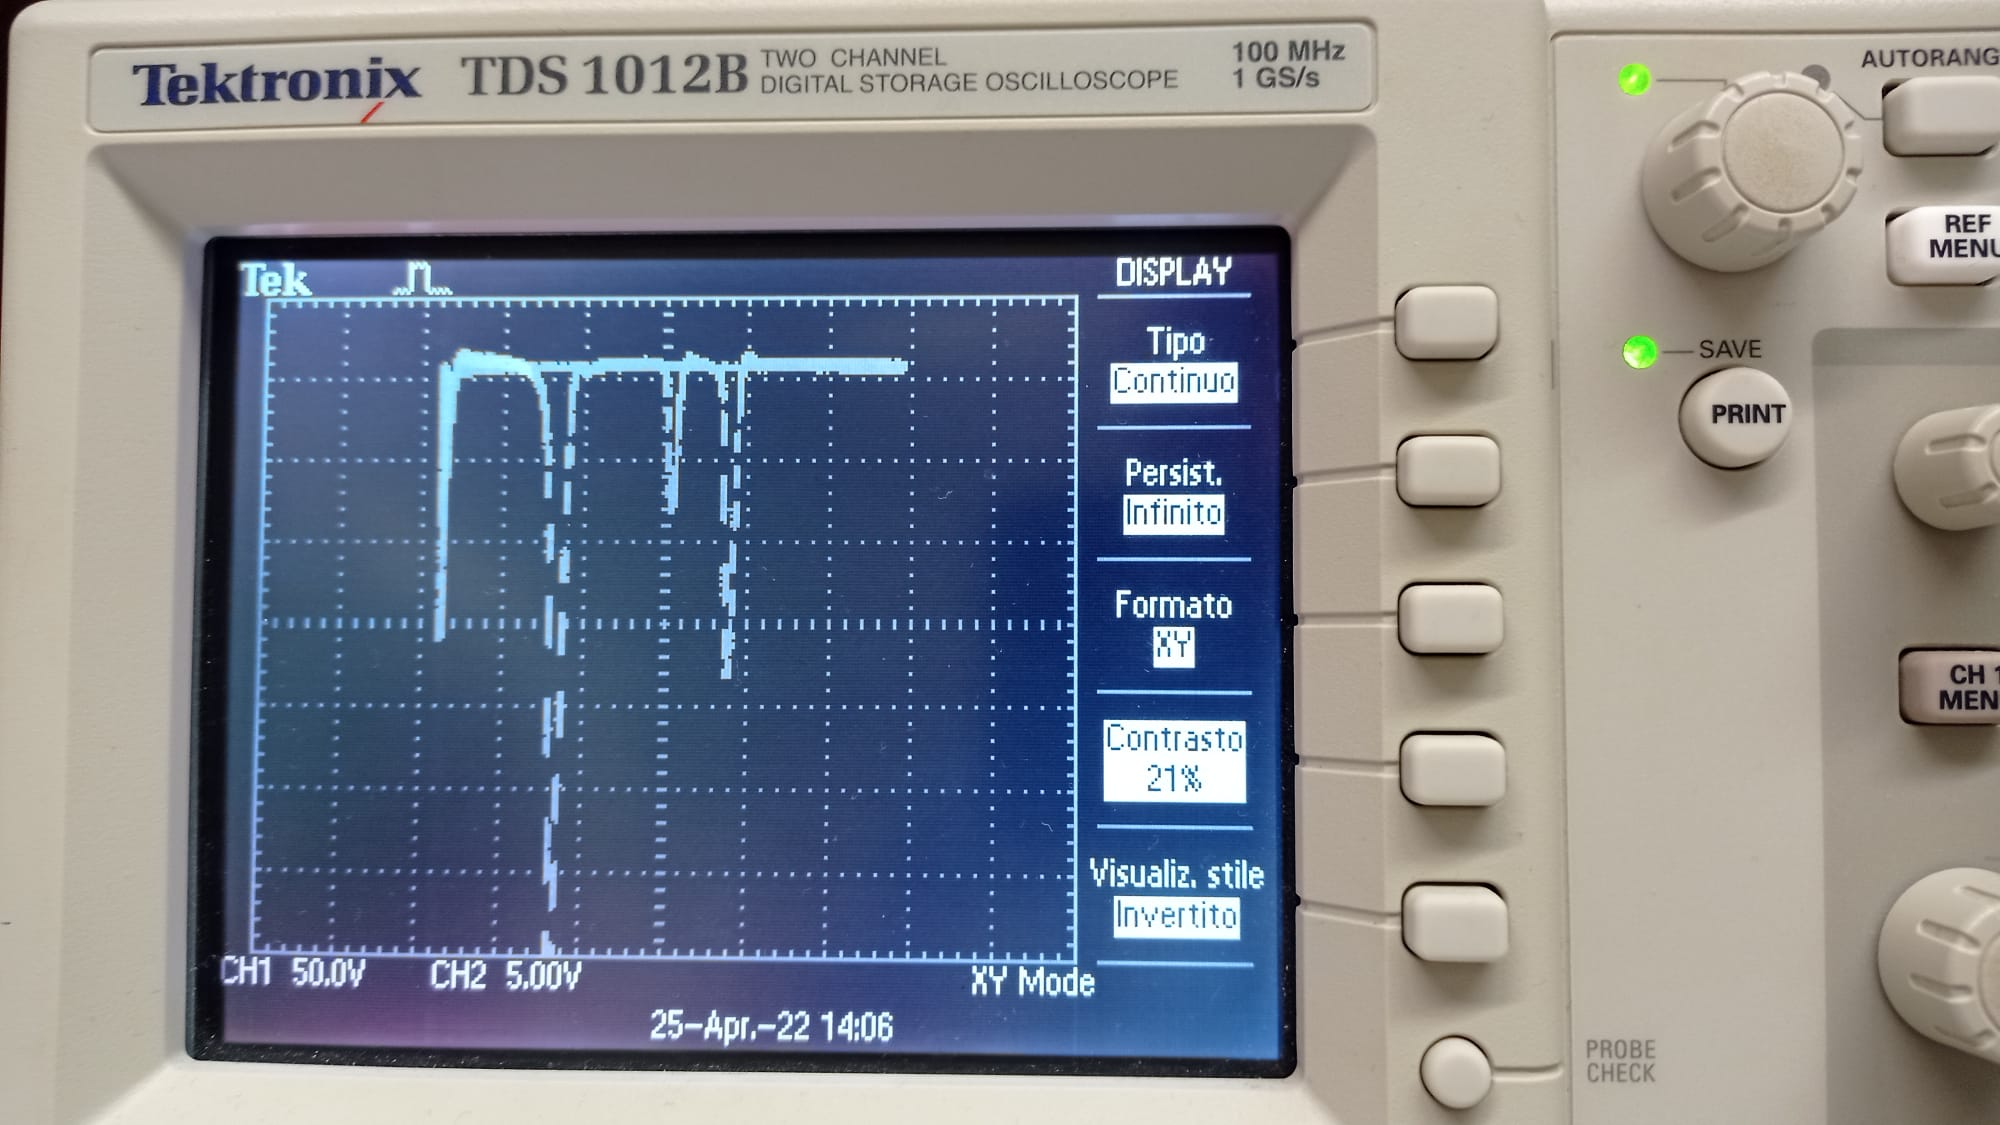
\includegraphics[width=0.6\textwidth]{latex/images/Messbild.jpeg}
			\caption{Ein typisches Oszilloskopbild der Transitivität gegen die horizontalkomponente des Magnetfeldes. 
			Der tiefste Peak auf der linken Seite des Bildes spiegelt die Stelle dar, andem die Horizontalmagnetfeldstärke 0 ist.
			Rechts daneben ist ein kleiner Peak, der durch die stimulierte Emission von Isotop 1 entsteht. 
			Der etwas größere Peak auf der rechten Seite entsteht durch die stimulierte Emission von Isotop 2.}
		\end{figure}	
	
	\subsection{Quadratischer Zeemann-Effekt}
